\section{Resultados}\label{sec:resultados}

\begin{frame}{Osciladores acoplados}
    \begin{minipage}{0.45\textwidth}
        \begin{block}{Parámetros variables}
            \begin{itemize}
                \item $k = 100\ kg/s^2$
                \item Se tomaron 5 valores de $\omega$ dentro del rango $[5, 15]$
                \item $dt = \min\left(10^{-3}, \frac{1}{100*\omega}\right)$
            \end{itemize}
        \end{block}
    \end{minipage}
    \hfill
    \begin{minipage}{0.45\textwidth}
        \centering{
            \begin{figure}[H]
                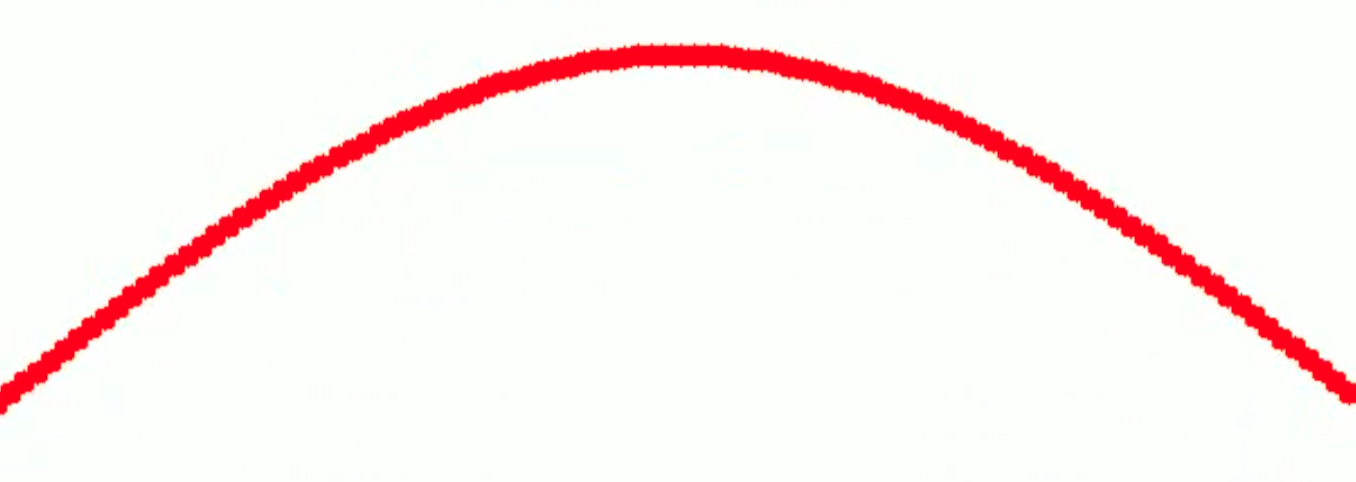
\includegraphics[width=1\textwidth]{pic/05-results/system_animation}
                \label{fig:system-animation}
            \end{figure}
            \tiny{\href{https://www.youtube.com/watch?v=GEmD58FVsSw}{https://www.youtube.com/watch?v=GEmD58FVsSw}}
        }
    \end{minipage}
\end{frame}

\begin{frame}{Osciladores acoplados}
    \textbf{Amplitud de oscilación del sistema}
    \begin{minipage}[c]{0.8\linewidth}
        \begin{figure}[H]
            \centering
            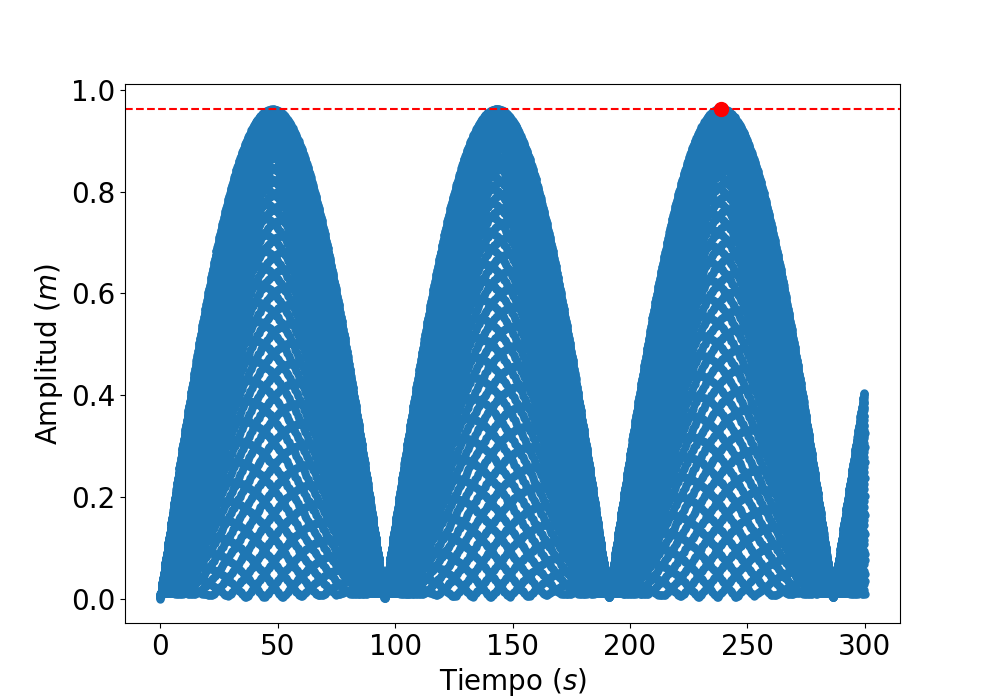
\includegraphics[width=0.8\textwidth]{pic/05-results/system_amplitude}
            \label{fig:system-amplitude}
        \end{figure}
    \end{minipage}
    \begin{minipage}{0.15\linewidth}
        \large{\text{$\omega = 10\ \frac{1}{s}$}}
    \end{minipage}
\end{frame}

\begin{frame}{Osciladores acoplados}
    \textbf{Máxima amplitud de oscilación del sistema}
    \begin{minipage}[c]{0.7\linewidth}
        \begin{figure}[H]
            \centering
            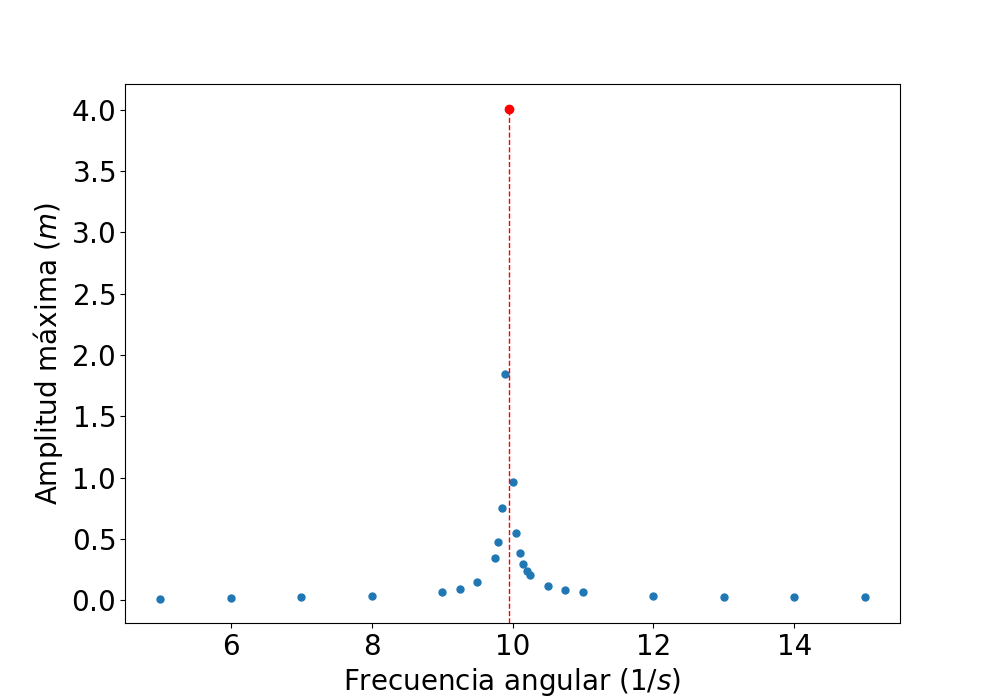
\includegraphics[width=0.8\textwidth]{pic/05-results/system_max_amplitude}
            \label{fig:system-max-amplitude}
        \end{figure}
    \end{minipage}
    \begin{minipage}[c]{0.25\linewidth}
        \large{
            \begin{equation*}
                \begin{aligned}
                    \omega_0 &= 9.95\ \frac{1}{s} \\ \\
                    H_{max}(\omega_0) &\approx 4.0095\ m
                \end{aligned}
            \end{equation*}
        }
    \end{minipage}
\end{frame}

\begin{frame}
    \begin{block}{Parámetros variables}
        \begin{itemize}
%            \item $k \in \left\{100 kg/s^2, 2500 kg/s^2, 5000 kg/s^2, 7500 kg/s^2, 10000 kg/s^2\right\} $
%            \item $\omega \in [5, 105]$
%            \item $dt = \min\left(10^{-3}\,s, \frac{1}{100 \omega}\,s\right)$
            \item $k=100 kg/s^2 $
                \begin{itemize}
                    \item Se tomaron 20 valores de $\omega$ dentro del rango $[5, 15]$
                \end{itemize}
            \item $k=2500 kg/s^2$
                \begin{itemize}
                    \item Se tomaron 20 valores de $\omega$ dentro del rango $[5, 15]$
                \end{itemize}
            \item $k=5000 kg/s^2$
                \begin{itemize}
                    \item Se tomaron 20 valores de $\omega$ dentro del rango $[5, 15]$
                \end{itemize}
            \item $k=7500 kg/s^2$
                \begin{itemize}
                    \item Se tomaron 20 valores de $\omega$ dentro del rango $[5, 15]$
                \end{itemize}
            \item $k=10000 kg/s^2$
                \begin{itemize}
                    \item Se tomaron 20 valores de $\omega$ dentro del rango $[5, 15]$
                \end{itemize}
        \end{itemize}
    \end{block}
\end{frame}

\begin{frame}{Analisis de $\omega_o$ variando $k$}
    \begin{minipage}[c]{0.65\linewidth}
        \begin{figure}[H]
            \centering
            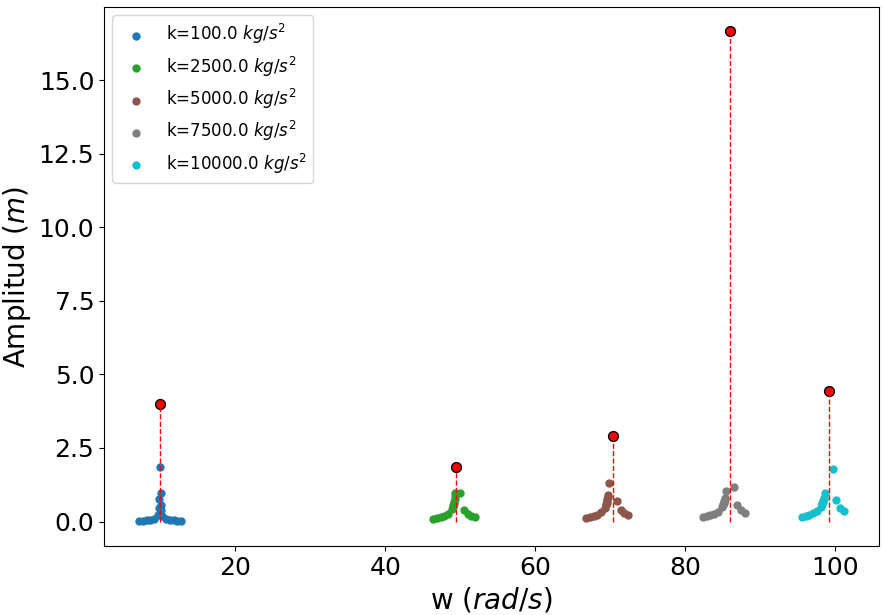
\includegraphics[width=1\textwidth]{pic/05-results/amp_w_k}
            \label{fig:amp_w_k}
        \end{figure}
    \end{minipage}
    \begin{minipage}[c]{0.34\linewidth}
        $dt = \min\left(10^{-3}\,s, \frac{1}{100 \omega}\,s\right)$
    \end{minipage}
\end{frame}

\begin{frame}{Analisis de $\omega_o$ variando $k$}
%    \begin{minipage}[c]{0.7\linewidth}
        \begin{figure}[H]
            \centering
            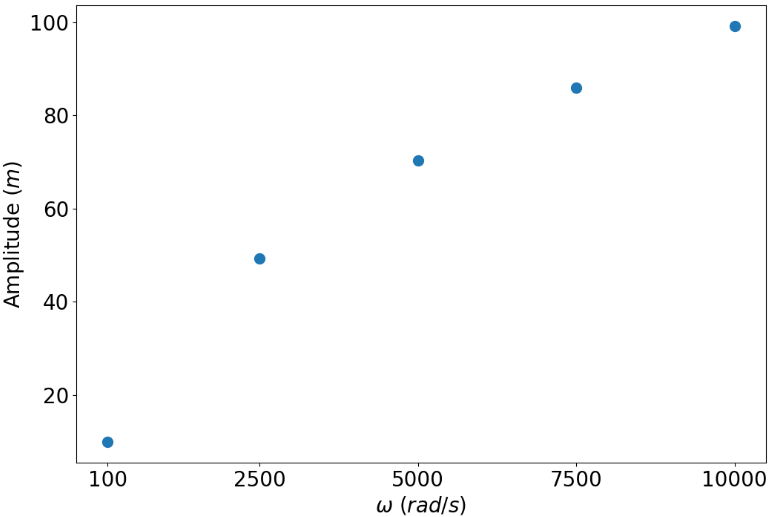
\includegraphics[width=0.7\textwidth]{pic/05-results/w_k}
            \label{fig:w_k}
        \end{figure}
%    \end{minipage}
%    \begin{minipage}[c]{0.25\linewidth}
%        \large{
%            \begin{equation*}
%                \begin{aligned}
%                    dt = \min\left(10^{-3}\,s, \frac{1}{100 \omega}\,s\right)
%                \end{aligned}
%            \end{equation*}
%        }
%    \end{minipage}
\end{frame}

\begin{frame}{Osciladores acoplados}
    \textbf{Ajuste lineal del factor de proporcionalidad}
    \begin{minipage}[c]{0.8\linewidth}
        \begin{figure}[H]
            \centering
            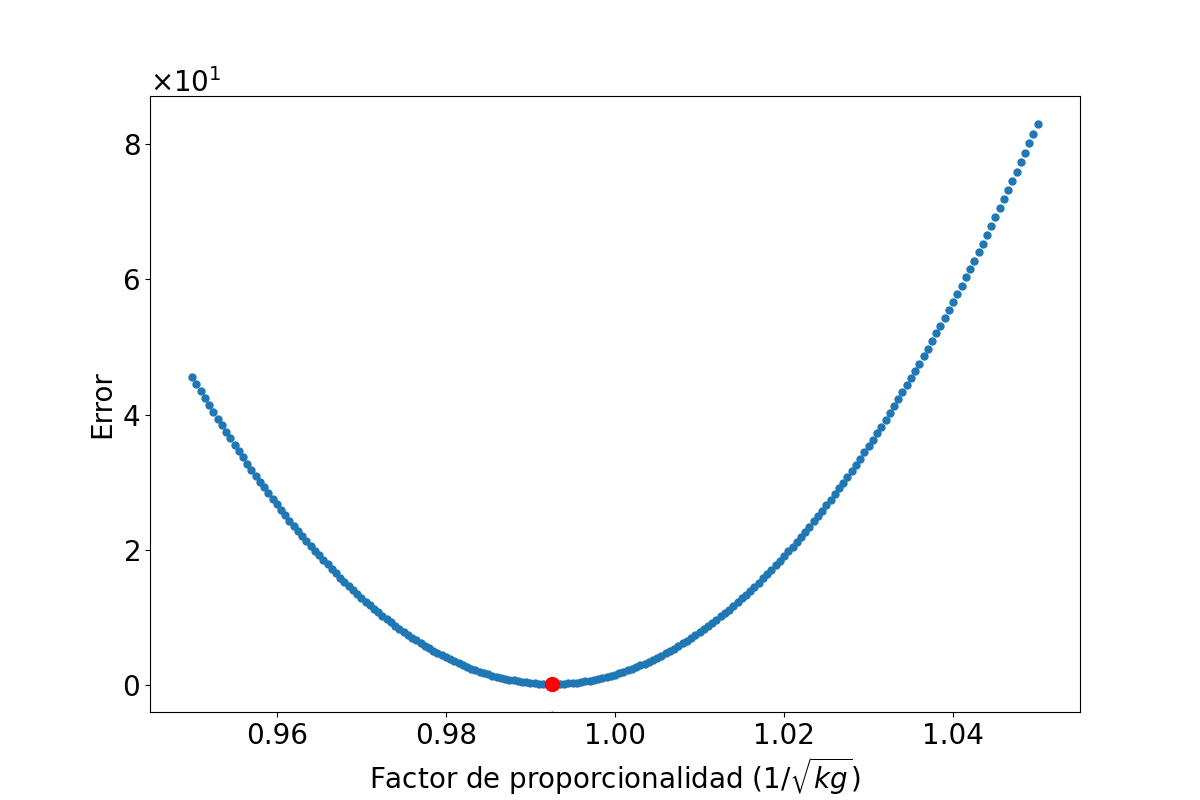
\includegraphics[width=0.8\textwidth]{pic/05-results/prop_error}
            \label{fig:prop-error}
        \end{figure}
    \end{minipage}
    \begin{minipage}{0.15\linewidth}
        \large{\text{$c = 0.9925\ \frac{1}{\sqrt{kg}}$}}
    \end{minipage}
\end{frame}

\begin{frame}{Osciladores acoplados}
    \textbf{Relación entre la frecuencia de resonancia y la constante elástica}
    \begin{figure}
        \centering
        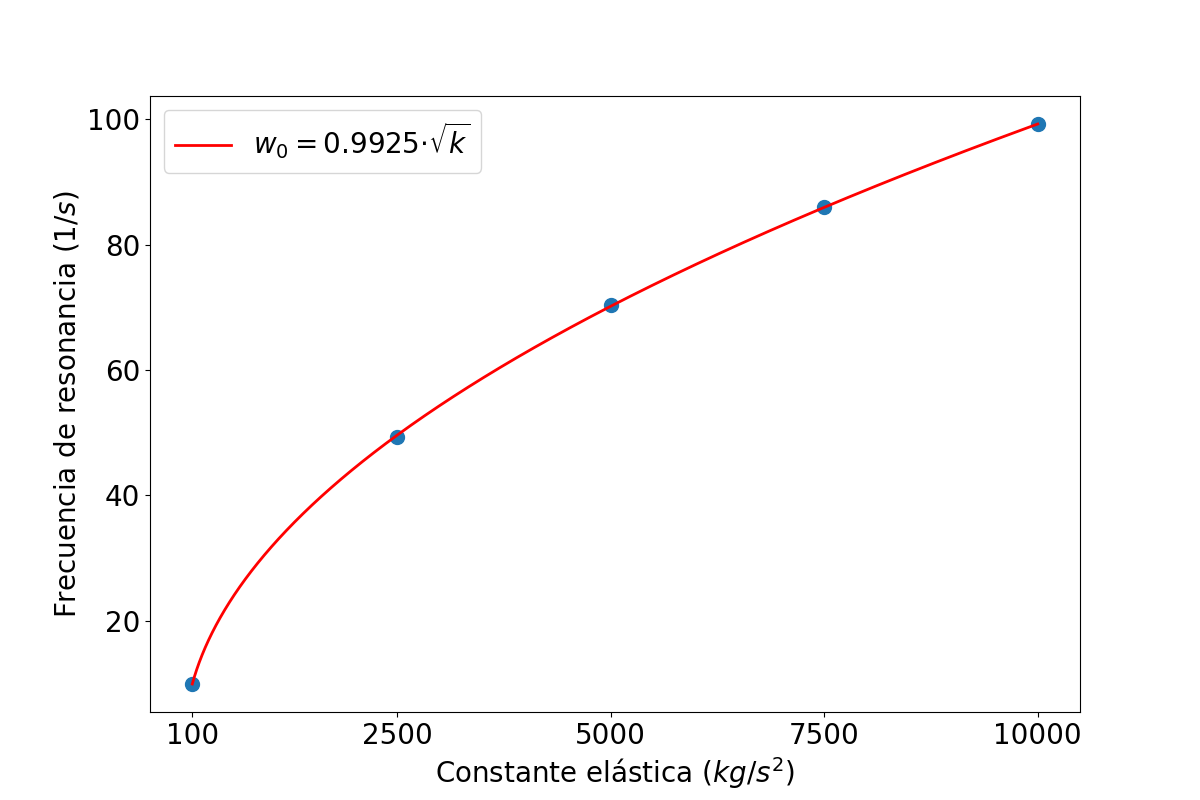
\includegraphics[width=0.7\textwidth]{pic/05-results/prop_relation}
        \label{fig:prop-relation}
    \end{figure}
\end{frame}